%%%%%%%%%%%%%%%%%%%%%%%%%%%%%%%%%%%%%%%%%
% Wenneker Article
% LaTeX Template
% Version 2.0 (28/2/17)
%
% This template was downloaded from:
% http://www.LaTeXTemplates.com
%
% Authors:
% Vel (vel@LaTeXTemplates.com)
% Frits Wenneker
%
% License:
% CC BY-NC-SA 3.0 (http://creativecommons.org/licenses/by-nc-sa/3.0/)
%
%%%%%%%%%%%%%%%%%%%%%%%%%%%%%%%%%%%%%%%%%

%----------------------------------------------------------------------------------------
%	PACKAGES AND OTHER DOCUMENT CONFIGURATIONS
%----------------------------------------------------------------------------------------

\documentclass[10pt, a4paper, twocolumn]{article} % 10pt font size (11 and 12 also possible), A4 paper (letterpaper for US letter) and two column layout (remove for one column)

%%%%%%%%%%%%%%%%%%%%%%%%%%%%%%%%%%%%%%%%%
% Wenneker Article
% Structure Specification File
% Version 1.0 (28/2/17)
%
% This file originates from:
% http://www.LaTeXTemplates.com
%
% Authors:
% Frits Wenneker
% Vel (vel@LaTeXTemplates.com)
%
% License:
% CC BY-NC-SA 3.0 (http://creativecommons.org/licenses/by-nc-sa/3.0/)
%
%%%%%%%%%%%%%%%%%%%%%%%%%%%%%%%%%%%%%%%%%

%----------------------------------------------------------------------------------------
%	PACKAGES AND OTHER DOCUMENT CONFIGURATIONS
%----------------------------------------------------------------------------------------

\usepackage[english]{babel} % English language hyphenation

\usepackage{microtype} % Better typography

\usepackage{amsmath,amsfonts,amsthm} % Math packages for equations

\usepackage[svgnames]{xcolor} % Enabling colors by their 'svgnames'

\usepackage[hang, small, labelfont=bf, up, textfont=it]{caption} % Custom captions under/above tables and figures

\usepackage{booktabs} % Horizontal rules in tables

\usepackage{lastpage} % Used to determine the number of pages in the document (for "Page X of Total")

\usepackage{graphicx} % Required for adding images

\usepackage{enumitem} % Required for customising lists
\setlist{noitemsep} % Remove spacing between bullet/numbered list elements

\usepackage{sectsty} % Enables custom section titles
\allsectionsfont{\usefont{OT1}{phv}{b}{n}} % Change the font of all section commands (Helvetica)

%----------------------------------------------------------------------------------------
%	MARGINS AND SPACING
%----------------------------------------------------------------------------------------

\usepackage{geometry} % Required for adjusting page dimensions

\geometry{
	top=1cm, % Top margin
	bottom=1.5cm, % Bottom margin
	left=2cm, % Left margin
	right=2cm, % Right margin
	includehead, % Include space for a header
	includefoot, % Include space for a footer
	%showframe, % Uncomment to show how the type block is set on the page
}

\setlength{\columnsep}{7mm} % Column separation width

%----------------------------------------------------------------------------------------
%	FONTS
%----------------------------------------------------------------------------------------

\usepackage[T1]{fontenc} % Output font encoding for international characters
\usepackage[utf8]{inputenc} % Required for inputting international characters

\usepackage{XCharter} % Use the XCharter font

%----------------------------------------------------------------------------------------
%	HEADERS AND FOOTERS
%----------------------------------------------------------------------------------------

\usepackage{fancyhdr} % Needed to define custom headers/footers
\pagestyle{fancy} % Enables the custom headers/footers

\renewcommand{\headrulewidth}{0.0pt} % No header rule
\renewcommand{\footrulewidth}{0.4pt} % Thin footer rule

\renewcommand{\sectionmark}[1]{\markboth{#1}{}} % Removes the section number from the header when \leftmark is used

%\nouppercase\leftmark % Add this to one of the lines below if you want a section title in the header/footer

% Headers
\lhead{} % Left header
\chead{\textit{\thetitle}} % Center header - currently printing the article title
\rhead{} % Right header

% Footers
\lfoot{} % Left footer
\cfoot{} % Center footer
\rfoot{\footnotesize Page \thepage\ of \pageref{LastPage}} % Right footer, "Page 1 of 2"

\fancypagestyle{firstpage}{ % Page style for the first page with the title
	\fancyhf{}
	\renewcommand{\footrulewidth}{0pt} % Suppress footer rule
}

%----------------------------------------------------------------------------------------
%	TITLE SECTION
%----------------------------------------------------------------------------------------

\newcommand{\authorstyle}[1]{{\large\usefont{OT1}{phv}{b}{n}\color{DarkRed}#1}} % Authors style (Helvetica)

\newcommand{\institution}[1]{{\footnotesize\usefont{OT1}{phv}{m}{sl}\color{Black}#1}} % Institutions style (Helvetica)

\usepackage{titling} % Allows custom title configuration

\newcommand{\HorRule}{\color{DarkGoldenrod}\rule{\linewidth}{1pt}} % Defines the gold horizontal rule around the title

\pretitle{
	\vspace{-30pt} % Move the entire title section up
	\HorRule\vspace{10pt} % Horizontal rule before the title
	\fontsize{16}{18}\usefont{OT1}{phv}{b}{n}\selectfont % Helvetica
	\color{DarkRed} % Text colour for the title and author(s)
}

\posttitle{\par\vskip 15pt} % Whitespace under the title

\preauthor{} % Anything that will appear before \author is printed

\postauthor{ % Anything that will appear after \author is printed
	\vspace{10pt} % Space before the rule
	\par\HorRule % Horizontal rule after the title
	\vspace{20pt} % Space after the title section
}

%----------------------------------------------------------------------------------------
%	ABSTRACT
%----------------------------------------------------------------------------------------

\usepackage{lettrine} % Package to accentuate the first letter of the text (lettrine)
\usepackage{fix-cm}	% Fixes the height of the lettrine

\newcommand{\initial}[1]{ % Defines the command and style for the lettrine
	\lettrine[lines=3,findent=4pt,nindent=0pt]{% Lettrine takes up 3 lines, the text to the right of it is indented 4pt and further indenting of lines 2+ is stopped
		\color{DarkGoldenrod}% Lettrine colour
		{#1}% The letter
	}{}%
}

\usepackage{xstring} % Required for string manipulation

\newcommand{\lettrineabstract}[1]{
	\StrLeft{#1}{1}[\firstletter] % Capture the first letter of the abstract for the lettrine
	\initial{\firstletter}\textbf{\StrGobbleLeft{#1}{1}} % Print the abstract with the first letter as a lettrine and the rest in bold
}

%----------------------------------------------------------------------------------------
%	BIBLIOGRAPHY
%----------------------------------------------------------------------------------------

\usepackage[backend=bibtex,style=authoryear,natbib=true]{biblatex} % Use the bibtex backend with the authoryear citation style (which resembles APA)

\addbibresource{example.bib} % The filename of the bibliography

\usepackage[autostyle=true]{csquotes} % Required to generate language-dependent quotes in the bibliography
\usepackage{datetime2}
 % Specifies the document structure and loads requires packages

%----------------------------------------------------------------------------------------
%	ARTICLE INFORMATION
%----------------------------------------------------------------------------------------

\title{Genomes of \textit{Wolbachia} endosymbionts from the human filarial parasites \textit{Mansonella perstans} and \textit{Mansonella ozzardi} reveal multiple origins of nematode-\textit{Wolbachia} symbiosis and convergent loss of bacterioferritin in filarial \textit{Wolbachia}} % The article title

\author{
	\authorstyle{
	Amit Sinha\textsuperscript{1},
	Zhiru Li\textsuperscript{1},
	Catherine B. Poole\textsuperscript{1},
	Laurence Ettwiller\textsuperscript{1},
	Natalie F. Lima\textsuperscript{2},
	Marcelo U. Ferreira\textsuperscript{2},
	Fanny F. Fombad\textsuperscript{3},
	Samuel Wanji\textsuperscript{3},
	Clotilde K.S. Carlow\textsuperscript{1}
	} % Authors
	\newline\newline % Space before institutions
	\textsuperscript{1}\institution{New England Biolabs, Ipswich, Massachusets 01938, USA}\\ % Institution 1
	\textsuperscript{2}\institution{Department of Parasitology, Institute of Biomedical Sciences, University of São Paulo, São Paulo, Brazil}\\ % Institution 2
	\textsuperscript{3}\institution{Department of Microbiology and Parasitology, University of Buea, Buea, Cameroon} % Institution 3
}

% Example of a one line author/institution relationship
%\author{\newauthor{John Marston} \newinstitution{Universidad Nacional Autónoma de México, Mexico City, Mexico}}

\date{\today} % Add a date here if you would like one to appear underneath the title block, use \today for the current date, leave empty for no date
%----------------------------------------------------------------------------------------

\begin{document}

\maketitle % Print the title

\thispagestyle{firstpage} % Apply the page style for the first page (no headers and footers)

%----------------------------------------------------------------------------------------
%	Record the date-time when the pdf was generated via compilation
%-------------------------------------------------------------------------
Compiled on {\ddmmyyyydate\today} at \DTMcurrenttime
%-------------------------------------------------------------------------


%----------------------------------------------------------------------------------------
%	Data Deposition Statement
%-------------------------------------------------------------------------
\section{Data deposition}
Raw Illumina reads for the M. perstans isolate Mpe1 and the M. ozzardi isolate Moz2 have been deposited in the NCBI SRA database under BioProject accession numbers PRJNA666672 and PRJNA666671 respectively. The assembled genome and PGAP annotations for the Wolbachia wMpe and wMoz are available from the NCBI GenBank database with accession numbers JACZHU000000000 and JADAKK000000000 respectively. The annotated genomes for wOcae and wMoviF are available as GenBank accessions JAHDJT000000000 and JAHRBA000000000 respectively, deposited under BioProject accessions PRJNA244005 and PRJNA739984 respectively.
%\raggedright

%----------------------------------------------------------------------------------------
%	ABSTRACT
%----------------------------------------------------------------------------------------
\section{Abstract}

\lettrineabstract{Mansonella ozzardi and Mansonella perstans, filarial parasites infecting millions of people worldwide, harbor their unique obligate endosymbionts, the alpha-proteobacteria Wolbachia wMoz and wMpe, respectively. Currently, little is known about these Wolbachia and no genome sequences are available. In the current study, high quality draft genomes of wMoz and wMpe were assembled from complex clinical samples using a metagenome assembly and binning approach. These represent the first genomes from supergroup F Wolbachia originating from human parasites and share features characteristic of filarial as well arthropod Wolbachia, consistent with their position in supergroup F. Metagenomic data analysis was also used to estimate Wolbachia titers, which revealed wide variation in levels across different clinical isolates, addressing the contradicting reports on presence or absence of Wolbachia in M. perstans. These findings may have implications for the use antibiotics to treat mansonellosis. Two additional supergroup F Wolbachia genomes, wOcae and wMoviF from arthropods Osmia caerulescens and Melophagus ovinus respectively, were assembled from publicly available raw Illumina reads in the NCBI SRA database. A phylogenomic analysis of Wolbachia genomes provides evidence for at least two independent events of horizontal transfer of Wolbachia from arthropod ancestors to filarial hosts within supergroup F. The analysis also uncovered a convergent pseudogenization and loss of the bacterioferritin gene in all filarial Wolbachia. Together, the wMoz and wMpe genome sequences provide a valuable resource for further studies on symbiosis, evolution and drug discovery.}

%----------------------------------------------------------------------------------------
%	ARTICLE CONTENTS
%----------------------------------------------------------------------------------------
%------------------------------------------------
\section{Introduction}

This sentence requires citation \citep{Reference1}. This sentence requires multiple citations to imply that it is better supported \citep{Reference2,Reference3}. Finally, when conducting an appeal to authority, it can be useful to cite a reference in-text, much like \cite{Reference1} do quite a bit. Oh, and make sure to check out the bear in Figure \ref{bear}.

Wolbachia are gram-negative $\alpha$-proteobacteria of the order Rickettsiales, present as intracellular symbionts in many species of parasitic filarial nematodes and arthropods1. While the Wolbachia associations in arthropods range from reproductive parasites to nutritional mutualists1,2, Wolbachia is an obligate mutualist in the filarial nematodes3 and is essential for worm development, fecundity and survival3,4. The latest phylogenetic classification, based on Multi-Locus Sequence Typing (MLST), assigns Wolbachia to various monophyletic supergroups5–7. Supergroups A, B, E, H and S are comprised entirely of arthropod Wolbachia, while supergroups C, D and J consist of filarial Wolbachia exclusively. Interestingly, the Wolbachia present in the filarial nematodes of the genus Mansonella are classified under supergroup F, the only supergroup to have Wolbachia members from nematode as well as arthropod hosts.
Mansonella perstans and Mansonella ozzardi are the two main causes of mansonellosis, and harbor their specific Wolbachia, wMpe and wMoz respectively. Mansonellosis is the most prevalent human filariases, yet the least studied and most neglected of all filarial infections8–13. M. perstans is considered to be the most common filaria in West and Central Africa9,12. It is also found in the Amazon rainforest and the Caribbean coast in South America12,14. M. ozzardi infections have been reported from many countries in South and Central America, including some Caribbean Islands10,12,15,16. Importantly, co-infections of M. perstans and M. ozzardi have been reported in South America17,18, making their treatment challenging as the two species respond differently to the commonly used anti-filarial drugs12. Antibiotics targeting Wolbachia have been successful in treating filarial diseases such as onchocerciasis and lymphatic filariasis4,19–24. Doxycycline, an effective anti-Wolbachia antibiotic, has been shown to clear M. perstans microfilariae12,25–27. Although no clinical trials have been reported, it is likley that antibiotics will have a similar effect against M. ozzardi28, enabling the use of a single drug to treat co-infections with M. ozzardi and M. perstans18. 
There is great interest in understanding the nature of the symbiotic relationship between Mansonella and their Wolbachia endosymbionts. The phylogenetic position of the Mansonella Wolbachia in a unique supergroup that also contains arthropod Wolbachia could also have implications for the nature of interactions with their host5,6,29,30. While genomic information could provide fundamental resource for investigating their biology, the only complete genome from supergroup F Wolbachia is the genome of Wolbachia from the bedbug Cimex lectularius (wCle)29. A draft genome of the supergroup F Wolbachia from Madathamugadia hiepei (wMhie), a filarial parasite of geckos, has become available recently6. However, since no genomic information is available for the Wolbachia of Mansonella, it is not known whether their biology is more closely aligned to filarial or arthropod Wolbachia12. 
Here, the first genomes of supergroup F Wolbachia wMoz and wMpe from human filarial parasites are reported. These draft genomes have been assembled from one isolate of M. ozzardi microfilariae from Venezuela, and one isolate of M. perstans from Cameroon. The genomes are slightly larger than 1 Mb and encode for about 900 genes each. The genome drafts are of high quality based on assessment of completeness using presence of conserved Wolbachia core genes as a metric. Analysis of deep-sequencing data from additional isolates of M. ozzardi and M. perstans provided some insights into the longstanding controversy around the status of Wolbachia across different Mansonella perstans isolates25–27,31–33. 
The Wolbachia members of supergroup F represent a unique opportunity to investigate and compare evolutionary trajectories of arthropod-Wolbachia versus filarial-Wolbachia symbiosis. For a comprehensive analysis of Wolbachia evolution, two additional genomes of supergroup F Wolbachia, wOcae and wMoviF, have been assembled from publicly available Illumina reads in the NCBI SRA database. The genomes of supergroup F Wolbachia from arthropod hosts Mengenilla moldryzki, Osmia caerulescens and Melophagus ovinus have been reported in literature (Gerth et al . 2014, Scholz et al. 2020) but are not available in GenBank. In this study, the corresponding Illumina data has been analyzed using a metagenomic approach to obtain the genomes for Wolbachia wOcae from O. caerulescens, and wMoviF from Melophagus ovinus. Additionally, a supergroup A Wolbachia was found to be present at low titers in M. ovinus. The genome of the Wolbachia from Mengenilla moldryzki could not be assembled most likely due to low sequencing coverage, and the metagenomic analysis revealed that the Wolbachia-like reads in this dataset is in fact originate from the regions of host genome that contain horizontally acquired Wolbachia sequences.
Phylogenomic analysis of all Wolbachia genomes from supergroup F revealed at least at least two independent origins of filarial-Wolbachia association, most likely from an ancestral arthropod-Wolbachia system. Additional phylogenomic analysis uncovered patterns of convergent gene losses and genome reduction in filarial Wolbachia as compared to the ancestral arthropod Wolbachia. One of the most striking examples is the loss of bacterioferritin gene from all filarial Wolbachia, with implications for biological role of Wolbachia in iron and heme metabolism of their hosts. 
In total, two filarial Wolbachia, wMoz and wMpe, and two arthropod Wolbachia, wOcae and wMoviF, are reported in this study, bringing up the number of supergroup F genomes from 2 (wCle and wMhie) to 6. The availability of the wMoz and wMpe genome sequences will provide further insight into the evolution and phylogenetic relationships of the Wolbachia endosymbionts of old and new world Mansonella species.  They will serve as an important resource for further studies on symbiosis, facilitate the development of improved methods for Wolbachia detection and contribute to the on-going search for new anti-Wolbachia drugs.

%------------------------------------------------
\section{Materials and Methods}
%------------------------------------------------

\subsection{Ethics statement}
All research involving human subjects was approved by the appropriate committee and performed in accordance with all relevant guidelines and regulations. Informed consent was obtained from all participants or their legal guardians.
For M. perstans, ethical clearance was obtained from the National Institutional Review board, Yaoundé (REF: N° 2015/09/639/CE/CNERSH/SP) and administrative clearance from the Delegation of Public Health, South-West region of Cameroon (Re: R11/MINSANTE/SWR/ RDPH/PS/259/382). Approval for the study was granted by the “National Ethics Committee of Research for Human Health” in Cameroon. Special consideration was taken to minimize the health risks to which any participant in this study was exposed. The objectives of the study were explained to the consenting donor after which they signed an informed consent form. The participant’s documents were given a code to protect the privacy of the study subject. At the end of the study, the donor received a cure of mebendazole (100 mg twice a day for 30 days).
For M. ozzardi, study protocols were approved by the Institutional Review Board of the Institute of Biomedical Sciences, University of São Paulo, Brazil (1133/CEP, 2013). Written informed consent was obtained from all patients, or their parents or guardians if participants were minors aged <18 years. Diagnosed infections were treated with a single dose of 0.2 mg/kg of ivermectin after blood sampling34,35.

\subsection{Parasite materials and DNA extraction}
DNA from M. ozzardi microfilariae from blood samples of individual subjects were collected as part of a previous study in Brazil35. One of the high microfilaremia samples was selected for genome sequencing and is denoted as Moz1 in the present study. A Venezuelan isolate of M. ozzardi microfilariae was generously donated by Izaskun Petralanda in 1989 and is denoted as Moz2 in this study. Genomic DNA was prepared from Moz2 microfilariae by Proteinase K digestion followed by phenol/chloroform extraction and ethanol precipitation, and drop dialysis (https://www.neb.com/protocols/2013/09/16/drop-dialysis) then stored at –20oC. Two independent isolates of M. perstans microfilariae, denoted as Mpe1 and Mpe2 in this study, were obtained on nylon filters from blood samples of consenting individuals in Cameroon36. Mpe1 DNA was extracted using a Genomic DNA Tissue MicroPrep kit (Zymo Research, USA) as described previously37. DNA from Mpe2 was isolated as described above for Moz2. DNA quantity was determined using a Qubit dsDNA HS Assay kit in conjunction with a Qubit 2.0 Fluorometer as directed by the manufacturer (Life Technologies, USA).

\subsection{Illumina library construction and sequencing}
The NEBNext Microbiome DNA enrichment kit (New England Biolabs Inc., USA) was used as directed to enrich for parasite DNA and reduce human DNA contamination prior to construction of the libraries from each of the samples, except Moz2. The preparation of Illumina libraries from Mpe1 and Moz1 samples have been described as part of a previous study37. A similar protocol was used for preparing libraries from Mpe2 and Moz2. Briefly, Illumina libraries were constructed using the NEBNext Ultra II FS DNA Library Prep Kit (New England Biolabs Inc., USA) as described by the manufacturer. Following PCR amplification with different index primers to enable multiplexing, the libraries were size selected using NEBNext Sample Purification Beads (NEB cat. # E7767) following manufacturer’s instructions. The approximate insert size and concentration of each library was determined using a 2100 Bioanalyzer with a high sensitivity DNA chip (Agilent Technologies, USA). Two Mpe2 libraries with insert sizes of approximately 500 and 800 bps and two Moz2 libraries with insert sizes of approximately 500 and 950 bps were constructed. Libraries were diluted to 4 nM with 10 mM Tris, 0.1 mM EDTA pH 8 for sequencing. Due to the A:T rich nature of filarial genomes, Phi X DNA was added to balance base pair composition, then sequenced using the Illumina MiSeq and NextSeq500 platforms (paired end, 150 bps). 

\subsection{Metagenomic assembly and binning}
Raw reads were processed using the BBTools package v38.51 (https://jgi.doe.gov/data-and-tools/bbtools/). Duplicate raw reads and bad tiles were removed using the clumpify.sh and filterbytile.sh utilities. Adapter trimming, removal of phiX reads and reads with 13-nt or longer stretches of the same nucleotide (poly-G, -C, -A or-T) was performed using bbduk.sh. Human host reads were removed by mapping against the human genome (grch38) using the bbmap.sh utility. The quality metrics of the processed reads at each step were assessed using FastqC v0.11.9 (https://www.bioinformatics.babraham.ac.uk/projects/fastqc/).
Reads from different runs of the libraries prepared from the same genomic DNA sample were combined and used as an input for the assembly of the metagenome using metaSpades v3.14.038. Input reads were mapped back to the assembled contigs using bowtie2 (v.2.4.1)39. Binning of metagenomic contigs into metagenome assembled genomes (MAGs) of Mansonella and Wolbachia was performed using the BlobTools v1.1.1 software40 and additional curation. The bins annotated as “Proteobacteria” and “Nematoda” were analyzed further to retrieve sequences originating from Wolbachia. A cluster of “Proteobacteria” contigs in the blobplots of each of the metagenomes was analyzed further using blastn against wCle genome to verify their Wolbachia origin. These contigs were subsequently collected as respective Wolbachia assemblies from each of the isolates. The combined size of contigs collected from the Moz1 isolate was only 120 kb, much smaller than a 1 Mb genome typically seen for Wolbachia and were not analyzed further. Similarly, in the Mpe2 sample, only 12 contigs with a total size of 15 kb were identified as candidate Wolbachia sequence and were not analyzed further. The tight clusters of “Proteobacteria” contigs in the blobplots of Moz2 and Mpe1 were analyzed further as the wMoz and wMpe genome assemblies respectively. For the remaining clusters of metagenome contigs that were marked also “Proteobacteria” by BlobTools but had a distinctly different %GC as compared to the Wolbachia contigs, blastn searches against the NCBI-nt database was performed to verify that they did not originate from the Wolbachia genome. All the bioinformatics programs were run using the default parameters unless otherwise stated.
The genome sequence of Wolbachia wOcae from the mason bee Osmia caerulescens was assembled from Illumina reads available under NCBI SRA accession SRR1221705 and originally described in a previous study of arthropod Wolbachia (Gerth et al. 2014). The reads were assembled into metagenomic contigs using metaSpades. A BlobTools analysis of the resulting assembly was used to identify the cluster of Wolbachia contigs. 
The genome sequence of Wolbachia wMoviF from the sheep ked Melophagus ovinus was assembled from raw Illumina reads corresponding to the NCBI SRA accession ERR969522, which originate form a study of sheep ked endosymbionts (Novakova et al. 2015) that were also used for Wolbachia genome mining in a recent research article (Scholz et al. 2020). In the first round of assembly using all reads as input to metaSpades assembler, potential Wolbachia scaffolds were identified using BlobTools. However, a preliminary blastn analysis of these scaffolds indicated the presence of a supergroup A or B Wolbachia in addition to the expected supergroup F Wolbachia in this sample. This was further corroborated by an analysis of protein coding genes predicted using PROKKA. A BUSCO analysis of these predicted genes revealed an unusually high proportion (17\%) of duplications of single copy orthologs conserved across Wolbachia, indicating the presence of at least two different Wolbachia in this host.  Therefore, due to the complicated nature of this dataset, additional iterations of metagenomic assembly and binning were performed using only the reads that mapped to a “bait” database containing all known Wolbachia genomes. The bait database was updated to include the newly assembled sequences, and the read filtering via mapping, followed by metagenomic assembly was repeated once more. The mapping of reads to bait databases was perform using bowtie2 v2.4.1 \underline{\textbf{\colorbox{Yellow}{(REF)}}}. Candidate Wolbachia scaffolds were selected using BlobTools. To separate the Wolbachia sequences originating from different supergroups, each scaffold was aligned to three representative and complete reference genomes, namely wCle (supergroup F), wMel (supergroup A), and wAlbB (supergroup B) using nucmer (command: nucmer -c 100 <ref\_genome> <query\_genome>), and the distribution patterns of sequence alignment, coverage scores and percentage identity scores was analyzed. The “affiliation score” of a particular scaffold to supergroup F versus supergroup A was calculated as the difference between its percent identity score to wCle and wMel. The histogram and density plot of the affiliation scores was plotted using R. The scaffolds with higher similarity to wCle were binned together as representing wMoviF, the supergroup F Wolbachia from M. ovinus, with the suffix F denotes the supergroup. A subsequent PROKKA and BUSCO analysis was used as a quality check to confirm that this bin did not contain a high proportion of duplicate single copy orthologs.
The raw Illumina reads used for obtaining the genome sequence of Wolbachia from the endoparasitic wasp Mengenilla modryzki correspond to the NCBI SRA accession SRR341096, which originate form a study of Strepsiptera genomes (Niehuis et al 2012) and had been used for Wolbachia analysis in a subsequent study (Gerth et al. 2014). The reads were assembled with metaSpades and BlobTools was used for obtaining the candidate Wolbachia scaffolds. However, the potential Wolbachia contigs were not well separated from the arthropod host scaffolds on the blobplot. For further investigation, PROKKA was used to predict protein coding genes on all the contigs. The taxonomic origin of each predicted gene was inferred via their closest seed ortholog in the eggNOG database as annotated by the eggNOG-Mapper pipeline. When the genes with seed orthologs in bacteria or arthropod were visualized on different tracks in IGV genome viewer (Thorvaldsdóttir and Mesirov 2013), Wolbachia-origin genes were found to be flanked by arthropod-origin genes. Therefore, no clear Wolbachia scaffolds could be identified in this dataset.


\subsection{Genome annotation and comparative analysis}
For both wMpe and wMoz genomes, as well as the wOcae and wMoviF genomes, protein-coding genes, rRNA, tRNA, ncRNA genes and pseudogenes were identified using the NCBI prokaryotic genome annotation pipeline41. Analysis of sequence similarity and synteny between wMoz, wMpe and wCle genomes was carried out using the JupiterPlot tool (https://github.com/JustinChu/JupiterPlot) which uses minimap242 for whole-genome alignments. The parameters used in Jupiter plots are maxGap = 100,000; minBundleSize = 1,000; m\_ref\_contig\_cutoff = 500; gScaff = 500. The parameter ‘ng’ was set to 100\%, so that all the contigs from the two assemblies being compared are displayed in the Jupiter plots. Whole-genome alignments of wMoz, wMpe as well as the wMhie genome against wCle as the reference genome were performed using the nucmer utility in MUMmer443 with default parameters. The resulting alignment blocks were visualized as concentric Circos plots44 drawn using the R package circlize v0.4.10 45. The completeness of the protein-coding content of all 4 genomes was assessed using the BUSCO pipeline v5.0 beta using the “proteobacteria\_odb10” reference dataset46. For global sequence comparisons across multiple Wolbachia genomes the average nucleotide identity (ANI) scores were calculated using the OrthoANIu tool v1.247. The pairwise ANI scores were used for hierarchical clustering of different Wolbachia, and a correlation plot was generated using R package corrplot v0.84 (https://github.com/taiyun/corrplot). For a more sensitive measure of sequence similarity and divergence between closely related Wolbachia, digital DNA–DNA hybridization (dDDH) scores48 were computed using the recommended “formula 2” at the “Genome-to-Genome Distance Calculator” (GGDC) web-service (https://ggdc.dsmz.de/ggdc.php). The orthologs of protein coding genes across multiple Wolbachia genomes were inferred using OrthoFinder v2.449, and the results visually represented as UpSet plots50 using the R package UpSetR v1.4.051. 
Insertion sequence (IS) elements were identified via the ISsaga web server52 and by parsing the annotations in GenBank format from NCBI-PGAP pipeline. Other transposons and Group II introns were also inferred via parsing the GenBank files. Phage-derived genes and regions were annotated by integrating the outputs from the PHASTER web server53, the PhiSpy v4.2.6 tool54 (https://github.com/linsalrob/PhiSpy/), and manual curation based on GenBank annotations. Functional annotation of protein-coding genes was carried out using the eggNOG-Mapper55 web server (http://eggnogdb.embl.de/\#/app/emapper). The analysis of different metabolic pathways was based on the annotations of wCle and wBm genomes available in the KEGG database56. 

\subsection{Phylogenomic analysis }
Phylogenomic analysis was carried out on different sets of input genomes. First, a preliminary tree was generated using 127 Wolbachia genomes, which include all the 123 annotated Wolbachia genomes available in NCBI GenBank database (Supplementary Table \underline{\textbf{\colorbox{Yellow}{XYZ}}}) and the 4 new genomes reported in this manuscript. Second, for a more robust and refined tree, any incomplete genomes, except the genomes within supergroup F were excluded from the analysis (Supplementary Table \underline{\textbf{\colorbox{Yellow}{XYZ}}}).  Also, redundant genomes e.g.  multiple isolates of the same Wolbachia but with no sequence differences were also excluded from this analysis, resulting in a total of 81 input genomes (Supplementary Table \underline{\textbf{\colorbox{Yellow}{XYZ}}}). Third, a high-resolution phylogenomic tree focusing only on genomes from supergroup F Wolbachia was generated, including the cat flea Wolbachia wCfeJ as an outgroup. 
For each of these phylogenomic analyses, a set of conserved Single Copy Orthologs (SCOs) present across all input genomes was identified using OrthoFinder. Protein sequences corresponding to each such orthogroup were aligned using mafft v\underline{\textbf{\colorbox{Yellow}{XYZ}}} \underline{\textbf{\colorbox{Yellow}{(REF)}}}. The multiple sequence alignments were trimmed using Gblocks \underline{\textbf{\colorbox{Yellow}{(REF)}}}. The trimmed bocks from each conserved orthogroup were then concatenated into a supermatrix, and the lengths of each alignment block was recorded in a nexus format partition file. The corresponding gene sequence tree was generated by collecting the transcript sequences corresponding to the single copy orthologs conserved all input Wolbachia. The DNA sequences corresponding to each conserved orthogroup were first aligned using mafft, and then concatenated into a supermatrix sequence, with the lengths of the alignment blocks recorded in a nexus format partition file. Maximum likelihood trees were generated based on protein sequences as well as gene sequences, using the corresponding supermatrix sequence and partition file as inputs to iqtree v\underline{\textbf{\colorbox{Yellow}{XYZ}}} \underline{\textbf{\colorbox{Yellow}{(REF)}}}.  Automatic selection of substitution models was performed using ModelFinder \underline{\textbf{\colorbox{Yellow}{(REF)}}} implementation in iqTree (iqTree command line option ‘-m MFP’). Evaluation of branch supports was performed using the iqTree implementations of (i) the SH-like approximate likelihood ratio test (Guindon et al., 2010), and (ii) ultrafast bootstrap with 1000 replicates each (iqTree command-line options ‘-B 1000 -alrt 1000 -abayes -lbp 1000’). The consensus trees were visualized using itol webserver \underline{\textbf{\colorbox{Yellow}{(REF)}}} and further annotated in Adobe Illustrator.     
For an expanded phylogenetic analysis covering all reported supergroup F Wolbachia, including those without whole genome sequences, their ftsZ gene sequence available in GenBank were utilized. The corresponding ftsZ sequence from wCfeJ was used as an outgroup. The ftsZ gene was chosen for this analysis from a list of candidate genes (ftsZ, groEL xxx , xxx) as this gene sequence was available for the highest number of supergroup F Wolbachia (Supplementary Table \underline{\textbf{\colorbox{Yellow}{XYZ}}}), second only to the 16S rRNA sequences. However, the trees based on 16S sequence were found to be not very informative due to the highly conserved nature of this region. The codons of ftsZ gene sequences were aligned using Muscle implementation in MEGAX v10.2.6 \underline{\textbf{\colorbox{Yellow}{(REF)}}} and gap regions were removed. A maximum likelihood tree was generated from this multiple sequence alignment using iqtree, with automatic selection of a codon substitution model. Bootstrap supports were calculated as described above.

\subsection{Gene loss and pseudogene analysis}
OrthoFinder results were analyzed to retrieve orthogroups that had gene members were present in all arthropod Wolbachia but not in filarial Wolbachia. In addition, then NCBI-PGAP annotations of supergroup F Wolbachia were analyzed to identify shared pseudogenes as follows. For each Wolbachia, the list of annotated pseudogene loci was extracted from the NCBI-PGAP annotations, and the loci derived from transposons and IS elements were excluded. The PGAP annotations also provide the GenBank accession of the most likely ancestral protein. The corresponding orthogroup for each of the ancestral protein was retrieved from the OrthoFinder results, thereby generating a list of orthogroups missing for each Wolbachia. The overlap between the missing orthogroups across different Wolbachia was analyzed and visualized using the R package UpsetR.

%------------------------------------------------

\section{Results}
\subsection{Metagenomic assembly and binning retrieves Wolbachia genomes from complex samples}
All four Mansonella isolates sequenced here were obtained as microfilariae from Mansonella-positive human subjects. The genomic DNA extracted from such clinical samples is unlikely to contain pure DNA originating from the parasite alone, instead each of the samples is expected to yield a complex assortment of mixed-organism DNA. The analysis of raw genome data from these samples therefore required a metagenomic assembly and binning approach to de-convolute parasite, symbiont and contaminants to permit species-specific genome assemblies. Further complicating correct assembly of Wolbachia genomes, is the presence of lateral gene transfer events where symbiont DNA can integrate into the nuclear genome of the host. Appropriate steps were taken to avoid including these HGT regions in the bacterial assemblies. 
	The assembled metagenome contigs were analyzed using BlobTools40, which is used to identify clusters of contigs based on their GC content, and read coverage obtained by mapping back input reads to the assembly, overlaid with sequence-identity based taxonomic classification. Partitioning the data in this manner generated distinct blobs corresponding to the desired target Wolbachia genomes from the mixed dataset, the genomes of the worm hosts and contaminating microbiota. (Supplementary Figure S1). The Wolbachia contigs identified from the BlobTools analysis were extracted as a separate bin of fasta sequences and analyzed further.
Of the two M. ozzardi isolates (Moz1 from Brazil and Moz2 from Venezuela), sufficient coverage was obtained from Moz2 that yielded a draft wMoz assembly of 1,073,310 bp in size comprised of 93 contigs. The N50 size of this assembly is 17.225 kb and the largest contig is 37.481 kb (Table 1). Of the two M. perstans isolates, Mpe1 and Mpe2, only Mpe1 yielded a Wolbachia assembly. The wMpe assembly is comprised of 1,058,123 bp in 170 contigs, with a N50 size of 10.041 kb and the largest contig is 28.485 kb (Table 1). 
The quality and correctness of these de novo assemblies were confirmed by various comparative analyses. Whole genome alignment of wMoz and wMpe visualized as a Jupiter plot demonstrates high sequence similarity and co-linearity of these independently assembled, closely related Wolbachia (Figure 1). A comparison was also made to the most closely related complete genome available in the Clade F supergroup, namely wCle, where high sequence synteny and co-linearity were also observed (Figures 2A and 2B). 
To determine the nature of the gaps in the draft assemblies, the whole genome alignments were investigated in more detail. Interestingly, most of the regions absent from wMoz and wMpe assemblies corresponded to regions containing IS element transposons in the wCle genome (Figure 3). A similar analysis using the draft genome of wMhie, the missing regions were again found to be associated with IS elements in wCle genome (Figure 3). Therefore, it appears that most of the protein coding regions have been recovered in these draft genome assemblies, and the missing regions mostly correspond to the IS elements. Due to their repetitive nature, IS elements are known to present a technical hurdle in assembling complete genomes, leading to fragmented assemblies57,58. 
Gene prediction using the NCBI PGAP pipeline identified 888 protein coding genes in wMoz and 864 protein coding genes in wMpe. A BUSCO analysis (v5.beta) was performed on these proteins, to check for presence of the 219 genes conserved across most proteobacteria (“proteobacteria\_odb10” database in BUSCO). The BUSCO scores of wMoz and wMpe were 77.6\% and 74.4\% respectively (Table 1), with such scores being typical for Wolbachia, even with complete genomes. For comparison, the corresponding scores for other Wolbachia were also calculated. The BUSCO scores for Wolbachia wOv from the human filarial parasite Onchocerca volvulus and wOo, present in the related bovine parasite Onchocerca ochengi are 76.7\% and 75.8\% respectively, and 79.5\% for wBm from the human filarial parasite Brugia malayi (Supplementary Figure S2). Within supergroup F, the BUSCO score for filarial Wolbachia wMhie is 79\% and is 81.7\% for the arthropod Wolbachia wCle. 

\subsection{Different isolates of Mansonella harbor varying levels of Wolbachia}
The metagenomic assembly and binning approach also enables the measurement of the relative amounts of Wolbachia in different isolates, by comparing the sequencing reads coverage of the Mansonella and Wolbachia specific contig bins in the metagenomic assemblies (Table 2). In the M. ozzardi sample (Moz2), the median coverage of contigs classified as Mansonella was observed to be 360X, while that of the Wolbachia contigs was found to be 13X. Assuming 1000 nematode cells per microfilaria59, each parasite is estimated to harbor 37 Wolbachia cells. For the other M. ozzardi isolate (Moz1) the median coverage for nematode contigs was only 57X and this low coverage is the most likely reason why this isolate did not yield sufficient Wolbachia contigs in its metagenomic assembly. Therefore, the titer calculations were not performed for the Moz1 isolate as they would not be robust at such low coverage and incomplete assembly. For the M. perstans sample (Mpe1), the median coverage of nematode contigs was 1032X and the Wolbachia coverage was 30X, yielding an estimated titer of 30 Wolbachia per microfilaria. In the other M. perstans isolate Mpe2, where only 12 Wolbachia contigs were produced in the metagenomic assembly, the median coverage for nematode contigs is relatively high 633X, indicating that the lack of Wolbachia contigs is not due to insufficient depth of coverage and is rather most likely due to a very low titer of Wolbachia in this sample. Since both isolates were collected in Cameroon, these observations point to variation in Wolbachia titers within the same species in a geographical area and could explain the conflicting reports on detection of Wolbachia in M. perstans25–27,31–33. 

\subsection{Two new genomes from supergroup F Wolbachia, wOcae and wMoviF from arthropod hosts}
For the Wolbachia wOcae from O. caerulescens, metagenomic assembly and binning was performed on Illumina sequencing reads (NCBI SRA accession SRR1221705) available from a previous study (Gerth et al. 2014). A BlobTools analysis of the assembled scaffolds identified a clear cluster of 186 Wolbachia contigs (Supplementary Figure \underline{\textbf{\colorbox{Yellow}{XYZ}}}) with a total size of 1.2 Mb, 899 protein coding genes and a BUSCO score of 79\% (Table 1). 
A first round of metagenomic assembly and analysis of Illumina reads from the sheep ked Melophagus ovinus provided multiple evidence supporting the presence of two different Wolbachia in this dataset.  First, a BlobPlot analysis identified almost 700 Wolbachia contigs adding up to a total size of 1.6 Mb, larger than any known Wolbachia genome so far. Second, the BUSCO analysis of the proteins predicted using PROKKA [REF] further revealed an unusually high proportion (17\%) of duplications of single copy orthologs conserved across Wolbachia. In the second round of metagenomic assembly, only the subset of reads that mapped to any of the known Wolbachia genomes was used as input iteratively, producing 572 Wolbachia scaffolds with a total size 1.48 Mb. Sequence similarity scores were calculated for each Wolbachia scaffold when compared wMel (supergroup A), wAlbB (supergroup B) and wCle (Supergroup F) using nucmer, and the distributions of was analyzed to identify the supergroup F Wolbachia sequences. The median of percentage identity and query-coverage scores for the scaffolds to wCle or wMel genomes was observed to be higher as compared to the wAlbB genome (Supplementary Figure S3A, B), indicating the presence of a supergroup F and a supergroup A Wolbachia. An affiliation score measuring the relative similarity to supergroup F was calculated for each scaffold, as the difference between its percentage identity to the wCle genome and the percentage identity to the wMel genome. This score showed a clear bimodal distribution, with a range from -15 to 13 and a median value of 6.4 (Supplementary Figure S3-C). The sequences with affiliation score greater than zero were classified as supergroup F Wolbachia (Supplementary Figure S3-C). Additionally, 40 scaffolds were found to have a nucmer hit only to the wCle genome and therefore included in the supergroup F bin. This Wolbachia has been named as Wolbachia wMoviF, where the suffix F denotes the supergroup. The final assembly size is 1.01 Mb, comprised of 196 scaffolds, a BUSCO score of 79\% , with no duplicated core genes. 
BlobTools analysis of metagenomic assembly from M. moldrzyki reads failed to find a cluster of Wolbachia scaffolds distinct from the arthropod scaffolds (Supplementary Figure S3E?). The BUSCO score for Proteobacteria core genes on the PROKKA gene predictions of this candidate Wolbachia scaffolds metagenome was very low (16.5\% complete, 18.7\% fragmented, 64.8\% missing) indicating the poor recovery of Wolbachia genome. Further, blastx analysis of the scaffolds identified regions with hits to Wolbachia proteins flanked by multiple arthropod protein hits on either side (Supplementary Figure S\underline{\textbf{\colorbox{Yellow}{XYZ}}}), indicating that these Wolbachia-like sequences originate from regions of HGT into the genome of the arthropod host. The median coverage of arthropod host scaffolds was \underline{\textbf{\colorbox{Yellow}{XYZ}}}x, indicating that even if this host harbors an endosymbiotic Wolbachia, the sequencing coverage is too low to recover its genome. The Wolbachia regions in this assembly display highest sequence similarity to supergroup F Wolbachia such as wCle [Supp Data to be shown?], indicating that these regions are acquired from a supergroup F Wolbachia. 

\subsection{Genome sequence comparisons between different Wolbachia}
Comparisons of sequence similarity and divergence between all supergroup F Wolbachia genomes, Wolbachia genomes from filarial nematodes, a plant parasitic nematode, and arthropod hosts representing different supergroups (Supplementary Table S1) were performed using the genome-wide average nucleotide identity (gANI) and digital DNA–DNA hybridization (dDDH) scores. The gANI scores (Figure 4A) for closely related sympatric Wolbachia are: 99\% for the wOo : wOv pair from Onchocerca spp. and 99\% for the wBm : wBpa pair from Brugia spp. Within supergroup F, highest gANI scores were observed to be 97\% between the wMoz : wMpe pair, and 92\% between wMoz : wCle and wMpe : wCle pairs (Figure 4A). wMhie shared a higher similarity with wCle (95\%), than to wMoz and wMpe (92\%). Comparisons between Clade F members and those of other clades generated gANI scores of a maximum value of 85\% (Figure 4A).

Using dDDH, a more sensitive metric for sequence divergence between very closely related species, the dDDH score of the wMoz : wMpe pair was found to be 71.7\% (Figure 4B). For comparison, the dDDH scores for other pairs of closely related Wolbachia are: 96.1\% for the wOo : wOv pair from Onchocerca spp. (Figure 4C) and 93.3\% for the wBm : wBpa pair from Brugia spp. (Figure 4D). Within supergroup F, the dDDH scores between filarial Wolbachia wMoz or wMpe and arthropod Wolbachia wMoviF and wOcae were surprisingly found to be higher (about 47\%) than the dDDH scores between filarial Wolbachia wMoz or wMpe and the filarial Wolbachia wMhie (around 45\%). For wMhie, the highest dDDH score, 61.80\% was observed when aligned to arthropod Wolbachia wCle.

\subsection{Phylogenomic analysis encompassing all Wolbachia genomes }
A total of 127 Wolbachia genomes, including 123 annotated genomes available from GenBank were used as input for a phylogenomic analysis (Supplementary Table \underline{\textbf{\colorbox{Yellow}{XYZ}}}). A core set of 46 Single Copy Orthologs (SCOs) present across all available genomes was identified using OrthoFinder and the corresponding phylogenetic tree was also produced as an output from OrthoFinder (supplementary Figure \underline{\textbf{\colorbox{Yellow}{XYZ}}}). For a further refinement of the tree, all incomplete or redundant genomes were excluded from analysis, except the genomes within supergroup F (Supplementary Table \underline{\textbf{\colorbox{Yellow}{XYZ}}}). OrthoFinder analysis on these selected 81 genomes identified 99 SCOs. A maximum likelihood tree with a partitioned model was built from the combined supermatrix of \underline{\textbf{\colorbox{Yellow}{XYZ}}} nucleotides (Figure 6) and \underline{\textbf{\colorbox{Yellow}{XYZ}}} amino acids (Supplementary Figure \underline{\textbf{\colorbox{Yellow}{XYZ}}}) from these 99 SCOs. 
The corresponding protein sequences from each Wolbachia were concatenated into a supermatrix that was used for multiple sequence alignment using MAFFT and poor-quality regions trimmed with GBlocks. The final concatenated alignment comprised of xxy,yzz amino acids and was used to infer a phylogenetic tree using iqTree, with automatic model selection and bootstrap replications posterior probability  also performed model selection and (Figure 6A). A similar analysis was performed using the DNA sequences of the 99 SCOs and . The resulting trees are in Figures 7B 

\subsection{Convergent loss of bacterioferritin across all filarial Wolbachia}
Genomes of filarial Wolbachia are typically smaller than arthropod Wolbachia. The analysis of orthology relationships across 81 Wolbachia genomes (Supp Table S\underline{\textbf{\colorbox{Yellow}{XYZ}}}), identified various classes of genes that are lost across all filarial Wolbachia but are present in arthropod Wolbachia. Repetitive and mobile genetic elements including IS elements and phage derived genes were observed at lower frequency in filarial Wolbachia, as previously described (Lefoulon et al 2020). The most striking pattern was observed for the gene bfr encoding for the Wolbachia bacterioferritin, which was found to be absent from all filarial Wolbachia. Further analysis identified pseudogene fragments of the bfr gene in various stages of degradation across filarial Wolbachia, revealed fragments of bacterioferritin gene in and pseudogenization. , or even completely absent in Wolbachia of supergroup C, from Onchocerca worms (Supplementary Figure S\underline{\textbf{\colorbox{Yellow}{XYZ}}}). Although the bacterioferritin locus in the RefSeq annotations of Wolbachia wBp from Brugia pahangi is not annotated as a pseudogene, a closer look at its sequence and multiple sequence alignment with other bacterioferritin genes indicates the loss of the canonical start codon ATG and a gain of an extra codon downstream (Supplementary Figure \underline{\textbf{\colorbox{Yellow}{XYZ}}}), suggesting the pseudogenization of this gene in wBp as well.  Within supergroup F, all filarial Wolbachia, namely wMoz, wMpe and wMhie contain a pseudogenized bacterioferritin, even though their most recent ancestors from arthropod Wolbachia have the corresponding gene intact. Since the wMoz-wMpe pair is placed in a separate clade from wMhie (Figure 6C), the bfr gene has been pseudogenized independently in the two separate lineages. 

\subsection{Biotin biosynthesis genes are absent in wMpe and wMoz as well as wMoviF and wOcae}
For a detailed functional analysis, the proteins encoded by the wMoz, wMpe, wMoviF and wOcae genomes were annotated using the eggNOG database (Supplementary Tables S4A-B). Additionally, biosynthetic pathway annotations for the wCle genome were obtained from the KEGG database and corresponding orthologs were identified in wMoz, wMpe wMoviF, wOcae and wMhie proteomes. 
The bedbug Wolbachia wCle genome harbors an operon encoding the enzymes involved in biosynthesis of biotin, supporting a nutritional mutualism between the bedbug and its Wolbachia29. Interestingly, this operon has most likely been laterally acquired by wCle from a co-infecting Rickettsia or Cardinium symbiont29. Given the paucity of genome data on other members of supergroup F, it is not clear whether this pathway is also present in other Wolbachia from this supergroup. Searches of the wMoz and wMpe proteomes did not reveal any members of the biotin biosynthetic pathway (genes bioA, bioD, bioC, bioH, bioF and bioB), suggesting that unlike the wCle and bedbug symbiosis, biotin supplementation is not the basis of mutualism between these Wolbachia and their filarial host (Supplementary Table \underline{\textbf{\colorbox{Yellow}{XYZ}}}) . These genes were also absent in the wMoviF and wOcae draft assemblies, indicating that biotin supplementation might be unique only to the bedbug and its Wolbachia association.  The absence of biotin pathway genes is unlikely to be due to the incomplete nature of the draft assemblies. Given the high BUSCO score (~80\%) of the assemblies, there is a high probability that at least fragments of a few of the 6 genes in the biotin pathway would have been detected if present in the genomes. Further, the biotin pathway genes were also found to be absent in the draft genome of wMhie - the other filarial Wolbachia from the supergroup F6. In contrast, the biosynthetic genes of other vitamin pathways present in wCle were easily found in wMpe, wMoz, wMoviF and wOcae (Supplementary Table S5A-E). 
The genes encoding members of various metabolic pathways characteristic of Wolbachia proteomes, namely the heme pathway, purine and pyrimidine biosynthesis pathways, riboflavin metabolism, and Type IV secretion systems were found to be mostly present in wMoz and wMpe (Supplementary Tables S5A-E). Ribosomal protein subunits, a common target for anti-Wolbachia drugs such as doxycycline, as well as candidate drug targets such as pyruvate phosphate dikinase (PPDK)60 were also present in both wMoz and wMpe. 

\subsection{Shared pseudogenes point to a common ancestor of wMoz and wMpe being present in the common ancestor of M. perstans and M. ozzardi}
Intracellular bacteria such as Wolbachia are expected to accumulate deleterious mutations over evolutionary timescales, with one consequence being the formation of pseudogenes61. Analysis of these pseudogenes can also shed light on the nature of genes that are dispensable during a symbiotic association with the host organism. Pseudogenes in wMoz (n = 145) and wMpe (n = 153) were annotated as a part of the NCBI PGAP pipeline and compared with corresponding annotations in wMhie (n = 137) and wCle (n = 224). These annotations include information on the ortholog of ancestral protein-coding gene for each pseudogene (Supplementary Table 6). If the same ancestral gene was found to be pseudogenized in two or more Wolbachia, it was counted as a shared pseudogene (Figure 6). Transposons such as IS elements were excluded from this analysis due to their tendency to frequently pseudogenize. 
For each Wolbachia, the majority of its pseudogenes were found to be unique to its genome, and only 1 pseudogene was shared among all the 4 Wolbachia. In pairwise comparisons of Wolbachia, only 2 to 7 pseudogenes were common among pairs of Wolbachia, except for the wMoz : wMpe pair, which share a much larger set (n = 38). This large proportion of common pseudogenes suggests that these pseudogenes were already present in the last common ancestor (LCA) of wMoz and wMpe.

\subsection{Mobile genetic elements and prophage remnants in wMoz and wMpe genomes}
Genes encoding various kinds of transposable elements, including IS elements, were identified based on annotation descriptions obtained from the PGAP pipeline. The wMoz genome assembly has 25 transposable elements (3 intact protein coding genes and 22 pseudogenes, Supplementary Table 3A), while the wMpe genome assembly contains 23 transposable elements (1 intact protein coding gene, 22 pseudogenes, Supplementary Table 3B). Applying the same search strategy to the wMhie genome assembly identified 66 transposon elements (16 intact protein coding genes, 50 pseudogenes, Supplementary Table 3C). Within the set of these transposable elements, the wMoz assembly harbors only 1 intact IS3 family gene and 12 pseudogenes from various families of IS elements. The wMpe draft genome contains 10 pseudogenes from various IS families but no intact IS element gene, while 14 intact and 42 pseudogenized IS elements were identified in the wMhie genome. Additional search for IS elements in wMoz and wMpe genome assemblies using the ISsaga web-server52 did not reveal any other IS elements in these genomes. In the complete wCle genome, ISsaga web-service could identify 149 IS elements, with the IS5 family being the most abundant (121 copies). The low number of IS elements observed in wMoz and wMpe is most likely due to the limitations of short-read data in capturing repeated elements. 
Group II introns are a common mobile element found in high copy numbers in many Wolbachia genomes, e.g. 53 copies in the wAlbB genome57. Both the wMoz and wMpe assembly contain only 1 pseudogene derived from a Group II intron, while no intact gene or pseudogene for these elements could be found in wMhie and wCle genomes as reported earlier6.
A search for prophage elements identified 9 phage derived genes in both wMoz and wMpe assemblies of which 4 have been pseudogenized in both Wolbachia (Supplementary Table 3D). A gene encoding gp6-like head-tail connector phage protein and a pseudogene derived from a phage portal protein were found only in wMoz, while a pseudogene derived from major tail-tube phage protein was found only in wMpe. This is in accordance with the trend of none or very few phage derived genes in filarial Wolbachia genomes6.

\begin{figure}
	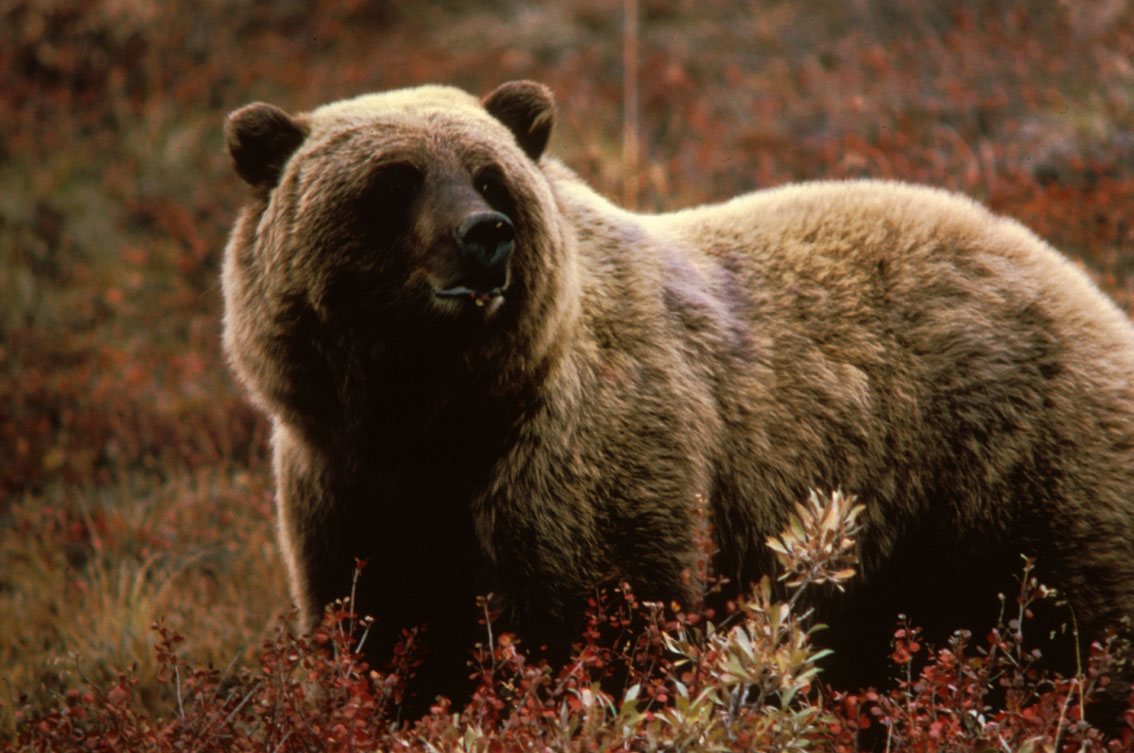
\includegraphics[width=\linewidth]{bear.jpg} % Figure image
	\caption{A majestic grizzly bear} % Figure caption
	\label{bear} % Label for referencing with \ref{bear}
\end{figure}

\section{Discussion}
To date, there are only two complete Wolbachia genomes available from human filarial parasites; wBm from Brugia malayi62, one of several parasites responsible for lymphatic filariasis or elephantiasis, and wOv from O. volvulus, the causative agent of onchocerciasis or river blindness63. These genomes belong to different phylogenetic lineages - wBm is a member of supergroup D, whereas wOv has been assigned to supergroup C. This is the first report describing the genomes of supergroup F Wolbachia from Mansonella. In this study a metagenomic approach was utilized to successfully retrieve the wMoz genome from one isolate of M. ozzardi collected in Venezuela and the wMpe genome from one isolate of M. perstans from Cameroon. The metagenomic assembly and binning approach that combines information from GC content of assembled contigs in conjunction with their read-coverage played a critical role in the generation of high-quality, draft genomes for wMpe and wMoz, from complex clinical samples containing a mixture of DNA from the human host, the filarial parasite and its intracellular symbiont and possibly other organisms that might be present in humans. The use of BlobTools40 for binning of contigs has been successfully employed previously to disentangle genomes of the Wolbachia wDimm from its host Dirofilaria immitis64,65, a filarial parasite of dogs and cats that occasionally infects humans. 
The metagenomic approach also enables an accurate determination of levels of endosymbiont present in the worm host. In a previous analysis of Wolbachia burden in different strains and stages of D. immitis, use of a BlobTools-like approach identified distinct blobs of contigs with levels of coverage consistent with high or low Wolbachia abundance65. Performing a similar analysis for Mansonella samples in the current study, the number of Wolbachia was estimated to be around 30 cells per microfilaria for samples Moz2 and Mpe1. This level of Wolbachia in Mansonella is considerably lower than the reported levels of 100 Wolbachia per microfilaria in Brugia malayi66. For the other M. perstans sample Mpe2 obtained from the same geographical location as Mpe1, only 12 small contigs corresponding to Wolbachia were found at very low coverage, demonstrating that the endosymbiont was present at extremely low levels, precluding accurate titer estimation. These observations indicate that even within a locality, Wolbachia levels can vary between different isolates, and could be a possible explanation for conflicting reports on the presence and absence of Wolbachia in M. perstans25–27,31–33. In addition to potential natural variation, previous exposure to antibiotics can also be a cause of very low Wolbachia levels and could be another explanation for the occasional failures to detect Wolbachia in PCR-based assays25–27,31–33. 
The observed differences in Wolbachia detection have raised doubts on the essentiality of Wolbachia in M. perstans32. However, the success of antibiotic treatments in reducing M. perstans microfilaremia supports an essential role of Wolbachia in this species25–27. Interestingly, Wolbachia has recently been reported in Mansonella sp. “DEUX” 33, a potentially new species of Mansonella parasite of humans, which is closely related to M. perstans67. To date, Wolbachia has been consistently found in all M. ozzardi isolates5,28, including the two isolates in the current study. Therefore, Wolbachia is most likely essential and present in all Mansonella parasites of humans, but can be present at different levels, sometimes below the limit of detection in M. perstans. 
The Wolbachia from supergroup F present a unique opportunity to investigate the evolutionary history of closely related arthropod and filarial Wolbachia. To enable such comparisons, two additional supergroup F genomes, wOcae and wMoviF, from arthropod hosts, have also been assembled in the current study. A phylogenomic analysis including the 4 genomes reported in this study, along with all the 123 Wolbachia genomes available in NCBI GenBank database confirmed their placement in the supergroup F. Further phylogenomic analysis of all supergroup F genomes revealed two independent origins of filarial Wolbachia within this supergroup, most likely from an ancestral arthropod Wolbachia. Since all other supergroups are comprised of either exclusively arthropod or filarial Wolbachia, the current phylogenetic analysis provides a first ever genomic support for the origin of filaria and Wolbachia symbiosis from ancestral arthropod hosts. These evolutionary scenarios have previously been proposed based on phylogenetic studies on a handful of genetic loci on a limited number of Wolbachia (Lefoulon et al. 2012). The genome-wide phylogeny based on \underline{\textbf{\colorbox{Yellow}{XYZ}}} nucleotides and \underline{\textbf{\colorbox{Yellow}{XYZ}}} amino acids incorporating 2 new filarial and 2 new arthropod Wolbachia genomes, provides the most comprehensive evidence in support of this hypothesis. A phylogenetic tree based on the ftsZ gene sequence also supports a clade of Mansonella Wolbachia separate from a clade with filarial Wolbachia wMhie and Wolbachia from the filarial parasite Cercopithifilaria japonica. 
Genome reduction and gene loss is a recurrent the in the evolution of endosymbionts \underline{\textbf{\colorbox{Yellow}{(REF)}}}, and the genomes of filarial Wolbachia are often found to be even more reduced as compared to their arthropod counterparts. A study of the genes lost during this evolutionary transition can therefore reveal genes that are dispensable for filaria - Wolbachia symbiosis. Gene loss was studied in using two approaches (1) looking at protein orthogroups that were present only on arthropod Wolbachia but in none of the filarial Wolbachia (ii) Direct comparison of annotated pseudogenes within supergroup F. The first approach revealed a striking loss of the bacterioferritin gene across in filarial Wolbachia across all supergroups (C, D, J and F). Within supergroup F, at least two independent losses of bacterioferritin gene were observed, one in the Mansonella Wolbachia clade and the other in the wMhie clade. Bacterioferritin is a critical storage compartment and regulator of heme metabolism \underline{\textbf{\colorbox{Yellow}{(REF)}}}, and the presence of an almost complete heme pathway in filarial worms has led to the hypothesis that heme supplementation by Wolbachia might be the basis of its obligate symbiosis with filarial nematodes, which lack the heme biosynthetic pathway (Foster et al. 2005, Gill et al. 2014). However, heme and iron metabolites can also be toxic to cells (Kremer et al. 2009?). In arthropods, Wolbachia symbionts protect their insect hosts from iron induced toxicity, and upregulate bacterioferritin expression to sequester excess iron/heme (Kremer et al. 2009). The lack of bacterioferritin in filarial Wolbachia suggests that the Wolbachia cells do not store heme, presumably to make it available to the host filaria. 
The four new genomes enable analysis of their evolutionary history from multiple perspectives. Insights can be gained from comparison of pseudogene content across different supergroup F Wolbachia. Since pseudogenes are evolutionary accidents, and the probability of such disruptions happening in the same gene in two independent lineages is low, the presence of multiple shared pseudogenes suggests that either these pseudogenes were already present in the last common ancestor (LCA) of wMoz and wMpe or are being lost due to convergent evolution. Since these endosymbionts are restricted to survive only within their host nematodes, it can be extrapolated that the LCA of wMoz and wMpe should have been already present in the last common ancestor of M. ozzardi and M. perstans. After the split, both wMoz and wMpe have continued to accumulate lineage-specific pseudogenes (n = 56 for wMoz, n = 62 for wMpe).
Orthology analysis and annotation of key biological pathways were performed to infer biological functions of the wMoz and wMpe endosymbionts. These comparisons included Wolbachia genomes from other filarial hosts, as well as representative genomes from other supergroups. Similar to other Wolbachia, genes encoding enzymes of various biosynthetic pathways, namely heme, purine, pyrimidine and riboflavin were present in wMoz and wMpe. The proposed anti-Wolbachia drug target PPDK involved in the glycolysis/gluconeogenesis pathway60 was conserved in all Wolbachia. Doxycycline, a commonly used anti-Wolbachia antibiotic that targets protein synthesis machinery, is reported to be effective against Mansonella perstans25–27. Consistent with this, all ribosomal subunits were found in wMoz and wMpe. 
The supergroup F Wolbachia wCle provides biotin as a nutritional supplement to its host bedbug and contains the complete pathway for biotin biosynthesis29 and has been acquired via LGT from another Rickettsia29. However, none of the genes of the biotin pathway could be found in wMoz, wMpe or in wMhie, indicating that biotin supplementation is not the basis of their filarial symbiosis. Further, the biotin pathway genes were not detected even in the arthropod Wolbachia wMoviF, wOcae.  Therefore, biotin pathway in the wCle genome is not a feature common to other Wolbachia of supergroup F.
In summary, high quality draft genomes of Wolbachia wMoz and wMpe from human filarial parasites M. ozzardi and M. perstans have been generated from genomic analysis of multiple isolates from different continents. Two additional genomes wMoviF and wOcae from arthropod Wolbachia from supergroup F have also been assembled from publicly available data, increasing the number of genomes in supergroup F from 2 to 6. These genomes provide an important resource for studies of symbiosis, evolution, comparative genomics, as well as searches for new drug targets. In addition, the successful use of a metagenomic assembly and binning approach for obtaining endosymbiont genomes exemplifies the wider applicability of this method to other systems where the DNA samples can only be obtained as complex mixtures of multiple organisms. Since the genomes from the host and endosymbiont are sequenced simultaneously, this approach uniquely enables a method for directly and robustly estimating the relative abundance of different organisms in a metagenomic sample. 

\section{Acknowledgements}
The authors thank Jeremy Foster for helpful discussions and comments on the manuscript, and Laurie Mazzola and Danielle Fuchs from the DNA sequencing core at New England Biolabs. The work was inspired by Don Comb and funded by New England Biolabs. Field research in Brazil was supported by the Fundação de Amparo à Pesquisa do Estado de São Paulo (FAPESP), research grant to M.U.F. (2013/12723-7) and doctoral scholarship to N.F.L. (2013/ 26928-0)

\section{Author Contributions}
N.F. L., M. U. F., F.F. F., S.W. collected the clinical samples. A.S., Z. L, C.B. P., L. E. performed the sequencing experiments and bioinformatics analysis. A.S., Z. L, C.B. P., L.E., C.K.S.C. analyzed the data. A.S., Z. L, C.B. P., C.K.S.C wrote the initial manuscript. A.S., Z. L, C.B. P., L.E., M. U. F., S.W., C.K.S.C and all authors contributed to the final manuscript.

\section{Tables}
\subsection{Table 1. Characteristics of genomes of wMoz and wMpe, and other Wolbachia from supergroup F}
Description needed??

\subsection{Table 2. Estimation of Wolbachia levels per microfilaria}
Description?

\section{Figure Legends}

\subsection{Figure 1. Schematic pipeline for metagenomic assembly and binning of supergroup F Wolbachia genomes}
The Wolbachia genomes assembly pipeline....

\subsection{Figure 2. Jupiter plot shows high concordance and synteny between the de novo assembled wMoz and wMpe genomes}
The Wolbachia genomes assembled from two biologically and geographically distinct isolates display a high level of synteny and inter-genome consistency. The genomes were aligned using minimap2 and visualized using the JupiterPlot software. The wMoz contigs are displayed as colored boxes in the left semi-circle, while the wMpe contigs are shown as gray boxes in the right semi-circle. The syntenic regions are marked by bands connecting contigs from one assembly to the corresponding region in the other assembly. Regions of rearrangement are shown as bands crisscrossing the horizontal bands of the syntenic regions.


\subsection{Figure 3. Jupiter plots show regions of conservation and synteny between (A) wMoz and (B) wMpe in comparison to the wCle genome}
The wCle chromosome is represented in linear form as the blue semi-circle on the left in both panels. The gray boxes represent contigs of (A) wMoz draft genome, and (B) wMpe draft genome. The horizontal bands connect the conserved regions across the two Wolbachia. Regions of re-arrangements are shown as bands crisscrossing the horizontal bands of syntenic regions. 

\subsection{Figure 4. Assembled draft genomes include most of the protein coding regions of Wolbachia, with the gaps corresponding to IS elements.}
missing from the draft genome assemblies of supergroup F Wolbachia correspond mostly to the IS elements
Whole genome alignments of wMpe (blue ring), wMoz (light-blue ring), wOcae (green ring), wMoviF (light green) and wMhie (innermost gray ring) to the wCle chromosome (outermost black circle) are visualized as a circos plot. The white bars mark the locations of the IS elements in the wCle genome. Compered to the 


\subsection{Figure 5. Global comparisons between multiple Wolbachia genomes using genome-wide Average Nucleotide Identity (gANI) scores, and digital DNA:DNA Hybridization (dDDH) scores. OR gANI and dDDH metrics to measure genome-wide sequence similarity between different  of Wolbachia}
(A) gANI scores were calculated between pairs of Wolbachia from filarial and plant-parasitic nematodes, and the arthropod Wolbachia wCle. Hierarchical clustering of pairwise gANI scores, presented as a correlation matrix, ordered the various Wolbachia in a pattern recapitulating their supergroup assignments. The red lines mark the boundaries between clusters representing different supergroups. (B) dDDH scores between members of supergroup F (C) dDDH scores between members of supergroup C, and (D) dDDH scores between members of supergroup D. 

\subsection{Figure 6. Phylogenomic analysis indicates multiple origins of filaria-Wolbachia endosymbiosis}
(A) Phylogenomic tree based on gene sequences of 91 single copy orthologs (SCOs) conserved across all Wolbachia. Supergroups with only arthropod hosts are marked in blue, filarial hosts are marked in orange, and supergroup F which has members from both arthropod and filarial hosts is marked in purple background. The red asterisks denote the Wolbachia with a pseudogenized  or absent bacterioferritin gene (B) The phylogenomic tree based on gene sequences of 525 SCOs conserved across all supergroup F Wolbachia indicates at least two independent origins of filaria-Wolbachia symbiosis, most likely from an arthropod-Wolbachia ancestor. The wMpe/wMoz lineage has split from the clade containing wOcae and wMoviF, while wMhie seems to be derived from a different ancestor that it shares with the bed bug Wolbachia wCle. The arthropod Wolbachia wCfeJ from the cat flea Ctenocephalides felis was used as the outgroup. (C) Phylogenetic tree of supergroup F Wolbachia based on ftsZ gene sequence also supports at least two independent origins of filarial Wolbachia. All Wolbachia from Mansonella hosts, including M. perforata are derived from a clade harboring arthropod Wolbachia wOcae and wMoviF, while the Wolbachia wMhie and wCjaponica from filarial hosts M. hiepei and Cercopithifilaria japonica fall in a separate clade more closely related the arthropod Wolbachia wCle.

\subsection{Figure 7. Venn diagram comparing pseudogenes in supergroup F Wolbachia}
Pseudogenes for wMoz and wMpe were annotated as a part of the NCBI PGAP pipeline. Transposons such as IS elements were excluded from this analysis due to their tendency to frequently convert into pseudogenes. 


\section{Supplementary Information}
\subsection{Figure S1. BlobTools based binning of the metagenomes assembled from Mansonella isolates (A) M. ozzardi isolate Moz1, from Brazil (B) M. ozzardi isolate Moz2, from Venezuela (C) M. perstans isolate Mpe1, from Cameroon and (D) M. perstans isolate Mpe2, from Cameroon.} 
Each dot in the plot represents a contig in the assembled metagenome, plotted by its \%GC content on the x-axis and log10 of its coverage on the y-axis. The dot size is scaled according to log10 of the length of each contig. Colors were assigned based on taxonomic annotations from BlobTools and manual annotations. Bins that were finally assigned to the Mansonella host and the Wolbachia endosymbiont are marked by enclosing boxes. Boxes with dashed borders indicate locations of expected Wolbachia contigs, but very few or very small contigs were actually recovered for these samples.

\subsection{Figure S2. BUSCO scores of various Wolbachia}
The BUSCO pipeline was used to measure the proportion of highly conserved, single copy orthologs (BUSCO groups). The set of reference BUSCO groups was set to the lineage “proteobacteria\_odb10”, which contains 219 BUSCOs derived from proteobacterial species. The wOo genome has the lowest BUSCO score, marked by a vertical dotted line. The supergroups are indicated within a parenthesis after the corresponding Wolbachia names.

\subsection{Table S1.} Wolbachia genomes used for comparative analysis with wMoz and wMpe genomes 

\subsection{Table S2: Orthology analysis using OrthoFinder} 
Table S2-A. Orthogroups and their member genes for different Wolbachia 
Table S2-B. Genes not assigned to any orthogroups.
Table S2-C. Overall OrthoFinder statistics for each Wolbachia genome analyzed.

\subsection{Table S3: Mobile genetic elements in wMoz and wMpe genome assemblies.} (A) Transposons and Group II introns in wMoz (B) Transposons and Group II introns in wMpe (C) Transposons in wMhie (D) Phage derived genes in wMoz and wMpe

\subsection{Table S4: eggNOG annotations of (A) wMoz and (B) wMpe proteins}

\subsection{Table S5: Various biological pathways in wMoz and wMpe and other supergroup F Wolbachia.}
(A) Heme pathway (B) Purine (C) Pyrimidine (D) Type IV and Type VI secretion systems

\subsection{Table S6: Pseudogenes present in the genomes of supergroup F Wolbachia}


%----------------------------------------------------------------------------------------
%	REFS PASTED FROM WORD
%----------------------------------------------------------------------------------------
\section{REFERENCESS PASTED FROM WORD}
%\begin{verbatim}
    
\begin{itemize}

\item 1.	Werren, J. H., Baldo, L. \& Clark, M. E. Wolbachia: master manipulators of invertebrate biology. Nat. Rev. Microbiol. 6, 741–751 (2008).
\item 2.	Zug, R. \& Hammerstein, P. Bad guys turned nice? A critical assessment of Wolbachia mutualisms in arthropod hosts. Biol. Rev. 90, 89–111 (2015).
\item 3.	Taylor, M. J., Bandi, C. \& Hoerauf, A. Wolbachia Bacterial Endosymbionts of Filarial Nematodes. in Advances in Parasitology (eds. Baker, J. R., Muller, R. \& Rollinson, D.) vol. 60 245–284 (Academic Press, 2005).
\item 4.	Pfarr, K. M. \& Hoerauf, A. M. Antibiotics which target the Wolbachia endosymbionts of filarial parasites: a new strategy for control of filariasis and amelioration of pathology. Mini Rev. Med. Chem. 6, 203–210 (2006).
\item 5.	Lefoulon, E. et al. Breakdown of coevolution between symbiotic bacteria Wolbachia and their filarial hosts. PeerJ 4, e1840 (2016).
\item 6.	Lefoulon, E. et al. Diminutive, degraded but dissimilar: Wolbachia genomes from filarial nematodes do not conform to a single paradigm. Microb. Genomics 6, e000487 (2020).
\item 7.	Lefoulon, E. et al. Pseudoscorpion Wolbachia symbionts: diversity and evidence for a new supergroup S. BMC Microbiol. 20, 188 (2020).
\item 8.	Downes, B. \& Jacobsen, K. A systematic review of the epidemiology of mansonelliasis. Afr. J. Infect. Dis. 4, (2010).
\item 9.	Simonsen, P. E., Onapa, A. W. \& Asio, S. M. Mansonella perstans filariasis in Africa. Acta Trop. 120, S109–S120 (2011).
\item 10.	Lima, N. F., Aybar, C. A. V., Juri, M. J. D. \& Ferreira, M. U. Mansonella ozzardi: a neglected New World filarial nematode. Pathog. Glob. Health 110, 97–107 (2016).
\item 11.	Mediannikov, O. \& Ranque, S. Mansonellosis, the most neglected human filariasis. New Microbes New Infect. 26, S19–S22 (2018).
\item 12.	Ta-Tang, T.-H., Crainey, J. L., Post, R. J., Luz, S. L. \& Rubio, J. M. Mansonellosis: current perspectives. Res. Rep. Trop. Med. 9, 9–24 (2018).
\item 13.	Bélard, S. \& Gehringer, C. High Prevalence of Mansonella Species and Parasitic Coinfections in Gabon Calls for an End to the Neglect of Mansonella Research. J. Infect. Dis. 223, 187–188 (2021).
\item 14.	Tavares da Silva, L. B. et al. Molecular Verification of New World Mansonella perstans Parasitemias. Emerg. Infect. Dis. 23, 545–547 (2017).
\item 15.	Raccurt, C. P. Mansonella ozzardi and its vectors in the New World: an update with emphasis on the current situation in Haiti. J. Helminthol. 92, 655–661 (2018).
\item 16.	Calvopina, M., Chiluisa-Guacho, C., Toapanta, A., Fonseca, D. \& Villacres, I. High Prevalence of Mansonella ozzardi Infection in the Amazon Region, Ecuador. 25, (2019).
\item 17.	Kozek, W. J., Palma, G., Henao, A., García, H. \& Hoyos, M. Filariasis in Colombia: Prevalence and Distribution of Mansonella Ozzardi and Mansonella (=Dipetalonema) Perstans Infections in the Comisaría Del Guainía. Am. J. Trop. Med. Hyg. 32, 379–384 (1983).
\item 18.	Crainey, J. L. et al. Deep-sequencing reveals occult mansonellosis co-infections in residents from the Brazilian Amazon village of São Gabriel da Cachoeira. Clin. Infect. Dis. Off. Publ. Infect. Dis. Soc. Am. (2020) doi:10.1093/cid/ciaa082.
\item 19.	Langworthy, N. G. et al. Macrofilaricidal activity of tetracycline against the filarial nematode Onchocerca ochengi: elimination of Wolbachia precedes worm death and suggests a dependent relationship. Proc. R. Soc. Lond. B Biol. Sci. 267, 1063–1069 (2000).
\item 20.	Bazzocchi, C. et al. Combined ivermectin and doxycycline treatment has microfilaricidal and adulticidal activity against Dirofilaria immitis in experimentally infected dogs. Int. J. Parasitol. 38, 1401–1410 (2008).
\item 21.	Taylor, M. J. et al. Preclinical development of an oral anti-Wolbachia macrolide drug for the treatment of lymphatic filariasis and onchocerciasis. Sci. Transl. Med. 11, (2019).
\item 22.	Clare, R. H. et al. Industrial scale high-throughput screening delivers multiple fast acting macrofilaricides. Nat. Commun. 10, 11 (2019).
\item 23.	Hübner, M. P. et al. In vivo kinetics of Wolbachia depletion by ABBV-4083 in L. sigmodontis adult worms and microfilariae. PLoS Negl. Trop. Dis. 13, e0007636 (2019).
\item 24.	Hong, W. D. et al. AWZ1066S, a highly specific anti-Wolbachia drug candidate for a short-course treatment of filariasis. Proc. Natl. Acad. Sci. 116, 1414–1419 (2019).
\item 25.	Keiser, P. B. et al. Molecular identification of Wolbachia from the filarial nematode Mansonella perstans. Mol. Biochem. Parasitol. 160, 123–128 (2008).
\item 26.	Coulibaly, Y. I. et al. A Randomized Trial of Doxycycline for Mansonella perstans Infection. N. Engl. J. Med. 361, 1448–1458 (2009).
\item 27.	Debrah, L. B. et al. The Efficacy of Doxycycline Treatment on Mansonella perstans Infection: An Open-Label, Randomized Trial in Ghana. Am. J. Trop. Med. Hyg. 101, 84–92 (2019).
\item 28.	Casiraghi, M., Favia, G., Cancrini, G., Bartoloni, A. \& Bandi, C. Molecular identification of Wolbachia from the filarial nematode Mansonella ozzardi. Parasitol. Res. 87, 417–420 (2001).
\item 29.	Nikoh, N. et al. Evolutionary origin of insect–Wolbachia nutritional mutualism. Proc. Natl. Acad. Sci. 111, 10257–10262 (2014).
\item 30.	Hosokawa, T., Koga, R., Kikuchi, Y., Meng, X.-Y. \& Fukatsu, T. Wolbachia as a bacteriocyte-associated nutritional mutualist. Proc. Natl. Acad. Sci. 107, 769–774 (2010).
\item 31.	Grobusch, M. P., Kombila, M., Autenrieth, I., Mehlhorn, H. \& Kremsner, P. G. No evidence of Wolbachia endosymbiosis with Loa loa and Mansonella perstans. Parasitol. Res. 90, 405–408 (2003).
\item 32.	Gehringer, C. et al. Molecular Evidence of Wolbachia Endosymbiosis in Mansonella perstans in Gabon, Central Africa. J. Infect. Dis. 210, 1633–1638 (2014).
\item 33.	Sandri, T. L. et al. Molecular Epidemiology of Mansonella Species in Gabon. J. Infect. Dis. 223, 287–296 (2021).
\item 34.	Basano, S. de A. et al. Phase III Clinical Trial to Evaluate Ivermectin in the Reduction of Mansonella ozzardi infection in the Brazilian Amazon. Am. J. Trop. Med. Hyg. 98, 786–790 (2018).
\item 35.	Lima, N. F., Gonçalves-Lopes, R. M., Kruize, Y. C. M., Yazdanbakhsh, M. \& Ferreira, M. U. CD39 and immune regulation in a chronic helminth infection: The puzzling case of Mansonella ozzardi. PLoS Negl. Trop. Dis. 12, e0006327 (2018).
\item 36.	Ritter, M. et al. Mansonella perstans microfilaremic individuals are characterized by enhanced type 2 helper T and regulatory T and B cell subsets and dampened systemic innate and adaptive immune responses. PLoS Negl. Trop. Dis. 12, e0006184 (2018).
\item 37.	Poole, C. B. et al. In Silico Identification of Novel Biomarkers and Development of New Rapid Diagnostic Tests for the Filarial Parasites Mansonella perstans and Mansonella ozzardi. Sci. Rep. 9, 10275 (2019).
\item 38.	Nurk, S., Meleshko, D., Korobeynikov, A. \& Pevzner, P. A. metaSPAdes: a new versatile metagenomic assembler. Genome Res. 27, 824–834 (2017).
\item 39.	Langmead, B. \& Salzberg, S. L. Fast gapped-read alignment with Bowtie 2. Nat. Methods 9, 357–359 (2012).
\item 40.	Laetsch, D. R. \& Blaxter, M. L. BlobTools: Interrogation of genome assemblies. F1000Research 6, 1287 (2017).
\item 41.	Tatusova, T. et al. NCBI prokaryotic genome annotation pipeline. Nucleic Acids Res. 44, 6614–6624 (2016).
\item 42.	Li, H. Minimap2: pairwise alignment for nucleotide sequences. Bioinformatics 34, 3094–3100 (2018).
\item 43.	Marçais, G. et al. MUMmer4: A fast and versatile genome alignment system. PLOS Comput. Biol. 14, e1005944 (2018).
\item 44.	Krzywinski, M. et al. Circos: An information aesthetic for comparative genomics. Genome Res. 19, 1639–1645 (2009).
\item 45.	Gu, Z., Gu, L., Eils, R., Schlesner, M. \& Brors, B. circlize Implements and enhances circular visualization in R. Bioinforma. Oxf. Engl. 30, 2811–2812 (2014).
\item 46.	Simão, F. A., Waterhouse, R. M., Ioannidis, P., Kriventseva, E. V. \& Zdobnov, E. M. BUSCO: assessing genome assembly and annotation completeness with single-copy orthologs. Bioinformatics 31, 3210–3212 (2015).
\item 47.	Yoon, S.-H., Ha, S., Lim, J., Kwon, S. \& Chun, J. A large-scale evaluation of algorithms to calculate average nucleotide identity. Antonie Van Leeuwenhoek 110, 1281–1286 (2017).
\item 48.	Meier-Kolthoff, J. P., Auch, A. F., Klenk, H.-P. \& Göker, M. Genome sequence-based species delimitation with confidence intervals and improved distance functions. BMC Bioinformatics 14, 60 (2013).
\item 49.	Emms, D. M. \& Kelly, S. OrthoFinder: phylogenetic orthology inference for comparative genomics. Genome Biol. 20, 238 (2019).
\item 50.	Lex, A., Gehlenborg, N., Strobelt, H., Vuillemot, R. \& Pfister, H. UpSet: Visualization of Intersecting Sets. IEEE Trans. Vis. Comput. Graph. 20, 1983–1992 (2014).
\item 51.	Conway, J. R., Lex, A., Gehlenborg, N. \& Hancock, J. UpSetR: an R package for the visualization of intersecting sets and their properties. Bioinformatics 33, 2938–2940 (2017).
\item 52.	Varani, A. M., Siguier, P., Gourbeyre, E., Charneau, V. \& Chandler, M. ISsaga is an ensemble of web-based methods for high throughput identification and semi-automatic annotation of insertion sequences in prokaryotic genomes. Genome Biol. 12, R30 (2011).
\item 53.	Arndt, D. et al. PHASTER: a better, faster version of the PHAST phage search tool. Nucleic Acids Res. 44, W16–W21 (2016).
\item 54.	Akhter, S., Aziz, R. K. \& Edwards, R. A. PhiSpy: a novel algorithm for finding prophages in bacterial genomes that combines similarity- and composition-based strategies. Nucleic Acids Res. 40, e126–e126 (2012).
\item 55.	Huerta-Cepas, J. et al. Fast Genome-Wide Functional Annotation through Orthology Assignment by eggNOG-Mapper. Mol. Biol. Evol. 34, 2115–2122 (2017).
\item 56.	Kanehisa, M., Furumichi, M., Tanabe, M., Sato, Y. \& Morishima, K. KEGG: new perspectives on genomes, pathways, diseases and drugs. Nucleic Acids Res. 45, D353–D361 (2017).
\item 57.	Sinha, A., Li, Z., Sun, L. \& Carlow, C. K. S. Complete Genome Sequence of the Wolbachia wAlbB Endosymbiont of Aedes albopictus. Genome Biol. Evol. 11, 706–720 (2019).
\item 58.	Lefoulon, E. et al. Large Enriched Fragment Targeted Sequencing (LEFT-SEQ) Applied to Capture of Wolbachia Genomes. Sci. Rep. 9, 1–10 (2019).
\item 59.	Basyoni, M. M. A. \& Rizk, E. M. A. Nematodes ultrastructure: complex systems and processes. J. Parasit. Dis. 40, 1130–1140 (2016).
\item 60.	Raverdy, S., Foster, J. M., Roopenian, E. \& Carlow, C. K. S. The Wolbachia endosymbiont of Brugia malayi has an active pyruvate phosphate dikinase. Mol. Biochem. Parasitol. 160, 163–166 (2008).
\item 61.	Andersson, S. G. E. \& Kurland, C. G. Reductive evolution of resident genomes. Trends Microbiol. 6, 263–268 (1998).
\item 62.	Foster, J. et al. The Wolbachia Genome of Brugia malayi: Endosymbiont Evolution within a Human Pathogenic Nematode. PLOS Biol. 3, e121 (2005).
\item 63.	Cotton, J. A. et al. The genome of Onchocerca volvulus, agent of river blindness. Nat. Microbiol. 2, 16216 (2016).
\item 64.	Kumar, S. \& Blaxter, M. L. Simultaneous genome sequencing of symbionts and their hosts. Symbiosis 55, 119–126 (2011).
\item 65.	Kumar, S., Jones, M., Koutsovoulos, G., Clarke, M. \& Blaxter, M. Blobology: exploring raw genome data for contaminants, symbionts, and parasites using taxon-annotated GC-coverage plots. Bioinforma. Comput. Biol. 4, 237 (2013).
\item 66.	McGarry, H. F., Egerton, G. L. \& Taylor, M. J. Population dynamics of Wolbachia bacterial endosymbionts in Brugia malayi. Mol. Biochem. Parasitol. 135, 57–67 (2004).
\item 67.	Mourembou, G. et al. Mansonella, including a Potential New Species, as Common Parasites in Children in Gabon. PLoS Negl. Trop. Dis. 9, e0004155 (2015).
\item 68.	Cerveau, N., Leclercq, S., Leroy, E., Bouchon, D. \& Cordaux, R. Short- and Long-term Evolutionary Dynamics of Bacterial Insertion Sequences: Insights from Wolbachia Endosymbionts. Genome Biol. Evol. 3, 1175–1186 (2011).

%\end{verbatim}
\end{itemize}

%----------------------------------------------------------------------------------------
%	BIBLIOGRAPHY
%----------------------------------------------------------------------------------------

\printbibliography[title={Bibliography}] % Print the bibliography, section title in curly brackets

%----------------------------------------------------------------------------------------

\end{document}
